\subsection{Worksheet - Lagrangians and Coordinate Transformations}
\begin{p}
If we transform $x, y$ into polar coordinates, what happens to the principle of least action? What do Lagrange’s equations become for a particle in a two-dimensional potential $U(x,y)$, now using polar coordinates. What are the generalized forces and generalized momenta? 
\end{p}
\begin{s}
Since the Lagrangian is invariant of the choice of coordinates, nothing happens; the principle of least action still holds (the Lagrangian and action integral are equivalent between the two coordinate systems):
\[S[r, \theta] = \int_{t_1}^{t_2}\LL(r, \dot{r}, \theta, \dot{\theta}, t)dt = \int_{t_1}^{t_2} \LL(x, \dot{x}, y, \dot{y}, t)dt = S[x, y]\]
Using the fact that $\v{r} = r\rhat$ and $\dot{\v{r}} = \dot{r}\rhat + r\dot{\phi}\phihat$ The Lagrangian becomes:
\[\LL = T - U = \frac{1}{2}m\dot{\v{r}}^2 - U(x,y) = \frac{1}{2}m(\dot{r}^2 + r^2\dot{\phi}^2) - U(r, \theta)\]
So Lagrange's equations become:
\[\dpd{\LL}{r} = \dod{}{t}\dpd{\LL}{\dot{r}} \implies -\dpd{U}{r} + mr\dot{\phi}^2 = m\ddot{r}\]
So the generalized force is $-\dpd{U}{r} + mr\dot{\phi}^2$ and the generalized momentum is $m\dot{r}$.
\[\dpd{\LL}{\phi} = \dod{}{t}\dpd{\LL}{\dot{\phi}} \implies -\dpd{U}{\phi} = mr^2\ddot{\phi}  \]
So the generalized force is $-\dpd{U}{\phi}$ (which is just the torque!) and the generalized momentum is $mr^2\dot{\phi}$ (which is the angular momentum!).
\end{s}

\begin{p}
Write the Lagrangian for two particles interacting through a potential $U(\v{r}_1, \v{r}_2)$, using the “lab frame” coordinates $\v{r}_1, \v{r}_2$. How does the potential simplify if it is translationally-invariant? How does it simplify if it is orientationally-invariant (i.e. central)? 
\end{p}
\begin{s}
The Lagrangian is given by:
\[\LL = \frac{1}{2}m_1\dot{\v{r}}_1^2 + \frac{1}{2}m_2\dot{\v{r}}_2^2 - U(x,y)\]
If the potential is translationally invariant, then there is no difference if we move the entire system through space; hence, it can only depend on the difference, i.e. $U(\v{r}_1 - \v{r}_2)$. If it is orientationally-invariant (central), then it only depends on the magnitude of the the difference, i.e. $U(\abs{\v{r}_1 - \v{r}_2})$.
\end{s}

\begin{p}
Rewrite the kinetic energy in terms of the centre of mass (CM) and relative coordinates, $\v{R}, \v{r}$. What are the Lagrange equations in these coordinates?
\begin{center}
    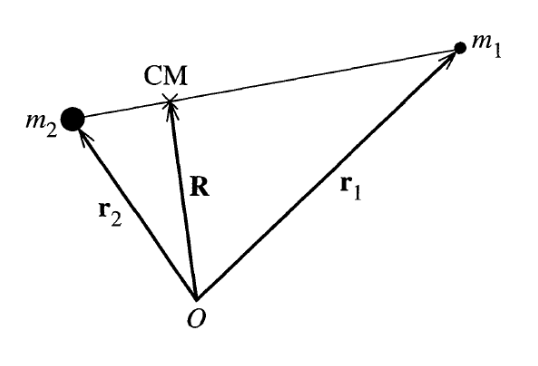
\includegraphics[scale=0.6]{Lecture-3/W3-img1.png}
\end{center}
\end{p}
\begin{s}
We have that the relative coordinate is $\v{r} = \v{r}_1 - \v{r}_2$ and $U = U(\abs{\v{r}})$. The CM position is given by:
\[\v{R} = \frac{m_1\v{r}_1 + m_2\v{r}_2}{m_1 + m_2}\]
Let us also define the combined mass $M = m_1 + m_2$, we then have that:
\[T = \frac{1}{2}\left(m_1\dot{\v{r}}_1^2 + m_2\dot{\v{r}}_2^2\right) = \frac{1}{2}\left(m_1\left(\dot{\v{R}} + \frac{m_2}{M}\dot{\v{r}}\right)^2 + m_2\left(\dot{\v{R}} - \frac{m_1}{M}\dot{\v{r}}\right)^2\right) = \frac{1}{2}\left(M\dot{\v{R}}^2 + \frac{m_1m_2}{M}\dot{\v{r}}^2\right)\]
So defining the reduced mass $\mu = \frac{m_1m_2}{M}$ we have:
\[\LL = T - U = \frac{M}{2}\dot{\v{R}}^2 + \left(\frac{\mu}{2}\dot{\v{r}}^2 - U(r)\right)\]
We end up with a Lagrangian that has essentially two independent terms; a COM motion term (which is trivial, just a particle of mass $M$) and a relative position term which is equivalent to a particle of mass $\mu$ subject to potential $U(r)$. We have essentially converted a two particle problem into what is effectively a one particle problem. This makes the two-body problem analytically (somewhat) easy to solve with this method.
\end{s}

\begin{p}
Write the expressions for $\v{r}_1$ and $\v{r}_2$ in terms of appropriate generalized coordinates, for the double pendulum. 
\begin{center}
    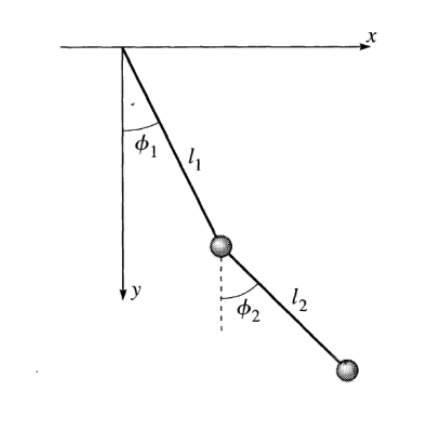
\includegraphics[scale=0.6]{Lecture-3/W3-img2.png}
\end{center}
\end{p}
\begin{s}
Trigonometry to get the position vectors:
\[\v{r}_1 = l_1\sin\phi_1\xhat + l_1\cos\phi_1\yhat\]
\[\v{r}_2 = \left(l_1\sin\phi_1 + l_2\sin\phi_2\right)\xhat + \left(l_1\cos\phi_1 + l_2\cos\phi_2\right)\yhat\]
This problem has four degrees of freedom (motion in the plane) but two constraints that $\abs{\v{r}_1} = l_1$ and $\abs{\v{r}_2 - \v{r}_1} = l_2$. This leaves to two generalized coordinates. Note that the constraints $f(\v{r}_1, \cdots, \v{r}_n, t) = 0$ are called "holonomic" and are in general nice for solving problems.
\end{s}